\section{Machine Learning}
\paragraph{Références} \cite{AlphaGo0} \cite{AlphaGo1} \cite{Internet3} \cite{Internet4} \cite{Internet5}

\paragraph{Une machine capable d'apprendre}

\paragraph {} Commençons par nous arrêter un instant sur le terme de \emph{Machine Learning}. En français,
cela pourrait se traduire par \emph{L'apprentissage de la machine}. Mais quel apprentissage ? N'est-ce pas
le rôle de l'Homme, comme nous l'avons soutenu jusqu'ici, d'apprendre à la machine ? Nous verrons que dans
le cas du Machine Learning, le concepteur ne fait que \emph{construire un système}, et lui donner
\emph{les clés} pour parvenir à la résolution d'un \emph{problème complexe}. On remarque ici l'importance
de \emph{cibler} un domaine: lorsque nous parlons de ML, nous ne prétendons pas créer un système à l'image
humaine, qui serait capable d'avoir une faculté d'apprentissage \emph{globale}, quelque soit le support. 

\paragraph{} Justement, n'est-ce pas là une réelle différence entre l'apprentissage humain et celui de la machine ?
Lorsque l'Homme apprend, c'est par \emph{l'expérience}. Il fait l'expérience de son environnement et la
conséquence de l'action lui permet d'être \emph{mieux préparé} à la prochaine expérience. Mais c'est en fait un
comportement similaire qui est utilisé en Machine Learning : un agent est entraîné à partir d'un certain nombre
d'entrées, dont il tire une sortie. Ce résultat est comparé à celui qui était attendu, puis la machine est
\emph{reparamétrée}, de sorte à ce qu'une prochaine expérience similaire aboutisse à un résultat plus proche 
de celui escompté. Ce processus de reconfiguration par l'apprentissage intervient notamment au niveau du cerveau
chez l'Homme, ce qui est concrétisé en, ML par l'utilisation de Réseaux Neuronaux ou Neural Networks (NN), dont
nous détaillerons l'utilisation par la suite. Ce qu'il faut retenir de la différence entre la méthode d'apprentissage
d'un Homme et d'une machine, c'est la capacité d'adaptation du tissu neuronal de l'Homme à une variété de situations
et de problèmes que la machine n'est pas capable d'appréhender seule.

\paragraph{Cerveau humain et Ordinateur}

\paragraph{} Afin de comprendre ces différences entre les capacités de l'Homme et de la machine, il nous faut nous
intéresser un instant à leur composition et à leur mode de fonctionnement. Rappelons en premier lieu qu'une machine
fonctionne sur un \emph{système binaire}, qu'elle est la seule à pouvoir comprendre. L'Homme de son côté réfléchit
par une infinité \emph{d'associations de sensations}, qui partent de son expérience sensorielle par les 5 sens : vue,
toucher, odorat, ouïe, goût. En ce sens la \emph{réflexion} est le propre de l'Homme, car il est seul à pouvoir 
apprendre par la projection de son expérience. \cite{Internet5}

\paragraph{} De plus, le cerveau humain possède une centaine de milliards de neurones, eux-mêmes connectés à plus de 10.000
de leurs voisins. Cette structure gigantesque n'est pas encore égalée par l'ordinateur, dont le nombre de cellules est de
l'ordre de 5 milliards, et dont les cellules sont contigües en mémoire. On remarquera néanmoins que l'information y circule
beaucoup plus rapidement que dans le cerveau, où les impulsions synaptiques atteignent 6 à 10 m/s. Enfin on remarquera que la
nature des mémoires est totalement différente : là où l'ordinateur est capable de \emph{stocker de l'information}, et est donc
capable de restituer une information de manière \emph{infaillible}, l'Homme doit compter sur les mémoires à court et long termes,
ainsi que sur ses registres sensoriels - ce qu'il connait de \emph{l'expérience}. \cite{Internet4}

\begin{figure}[h]
    \centering
    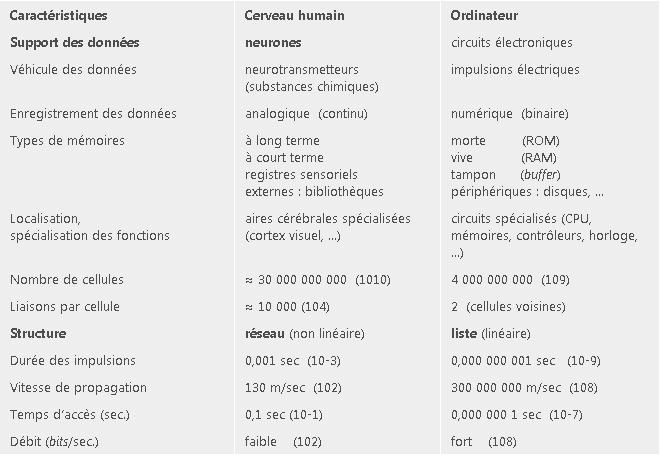
\includegraphics[width=350px]{chapters/03/images/cerveau-robot.jpg}
    \caption{\label{comparatif} \emph{Comparaison entre cerveau humain et ordinateur}, \url{http://intelligence-artificielle-tpe.e-monsite.com/pages/limites-technologiques-et-ethique-de-l-ia/cerveau-humain-et-robot.html}}
\end{figure}

\paragraph{Résoudre des problèmes complexes}

\paragraph{} Pour mettre en avant la valeur ajoutée du Machine Learning, nous allons nous intéresser à l'exemple pertinent
du possesseur du chat appellé Ada \cite{Internet3}. Il tente de poser la question suivante : qu'est-ce qu'Ada essaie de dire
à son maître lorsqu'elle ronronne quelques instants après avoir fait tomber la télécommande de la table basse ? Cela ne semble
pas avoir de réponse absolue en premier lieu, car il n'est pas possible de \emph{parler la langue d'Ada}, si tant est qu'on puisse
parler le chat.. De fait, nous cherchons donc une réponse \emph{appropriée}, c'est-à-dire au plus proche des attentes qu'avait eu
Ada auparavant, quand \emph{elle avait ronronné de la manière}, ou \emph{dans un contexte similaire}. Une multitude de réponses
possibles s'ouvrent alors à nous : elle à peut-être faim, ou encore elle cherche de l'attention, ou bien elle n'aime pas les
télécommandes, ou elle aime simplement faire tomber des objets.. 

\paragraph{} Néanmoins, les ordinateurs font d'ores et déjà un nombre incalculable de choses que nous ne serions pas capables de faire
par nous-même comme la navigation, le calcul, le monitoring... serait-il donc possible que l'on construise un logiciel qui résolve le problème
d'Ada pour nous ? Cette question est fondamentale car elle nous demande de savoir si un ordinateur est capable d'apprendre à un résoudre un
problème \emph{quelconque et indéterminé}. Si un logiciel peut comprendre Ada à partir de son observation, alors nous en déduisons qu'il devrait
être possible de lui donner n'importe quel système à observer afin qu'il puisse répondre à ses attentes.   

\paragraph{L'approche \emph{classique}} Afin d'écrire le logiciel qui répondrait au problème d'interprétation d'Ada, un développeur commun,
non initié au ML, devrait partir d'un ensemble de règles, parfaitement détaillées. Cela devrait reprendre tous les sons possibles émis par Ada,
les interprétations de ses comportements, de ses gestes, en fonction éventuellement du lieu, de la période... Tout cela afin de parvenir au 
\emph{message} qu'Ada est actuellement en train de transmettre. En somme, il faut arriver à figurer parfaitement, sous la forme de règles,
la représentation d'un problème particulier pour aboutir à la solution correcte. C'est-à-dire que le développeur devrait \emph{comprendre parfaitement}
Ada afin que l'ordinateur puisse atteindre la même compréhension, or nous réalisons bien que c'est impossible.

\paragraph{} Ce qu'il faut comprendre ici, c'est simplement que l'humain est \emph{faillible}. Il est toujours \emph{possible} qu'il se trompe
ou qu'il n'ait pas considéré les variables \emph{dans leur ensemble}. Ce n'est pas un mal en soi, et c'est bien le fait d'avoir accepté cette
faiblesse de l'humain par rapport à la machine qui lui a permis de remplacer l'un par l'autre dans des domaines où l'erreur n'est pas possible.
Il nous est impossible aujourd'hui d'imaginer la gestion des transports sans informatique, la santé sans matériel haute technologie afin de
permettre des analyses poussées, ou encore la finance sans tout le support des machines qui permettent notamment \emph{l'existence des marchés}. 

\paragraph{Une solution: le Machine Learning} Là où l'humain ne peut pas conçevoir la complexité liée à la compréhension d'Ada, il semblerait que les
ordinateurs puissent eux approcher une solution exploitable. D'ordinaire, afin de résoudre des problèmes, les ordinateurs utilisent des \emph{affectations}
(\emph{mapping}) de questions ou problèmes (en entrée) à des réponses ou solutions (en sortie). Tout le principe réside dans les étapes à respecter lors de
cette affectation, et nous avons pu voir qu'un développeur n'a pas toujours la réponse à cette question. De fait, pourquoi ne pas demander à une 
machine de se rendre compte \emph{elle-même} de la meilleure manière de faire cette affectation ? \cite{Internet3} C'est exactement le propos du Machine
Learning. Il s'agit en général de renseigner \emph{d'immenses quantités} de données du problème afin qu'il adopte l'algorithme qui répond le mieux à
comment configurer ce \emph{mapping}. Cela est rendu possible, comme nous l'avons vu précédemment dans la section sur \emph{le cerveau et l'ordinateur},
par l'immense faculté de calcul \emph{infatiguable} et \emph{infaillible} de la machine.

\paragraph{Sélectionner les données} Lorsque nous avons abordé le sujet de la collecte des données plus tôt, nous avons rapidement constaté la 
multiplication \emph{exponentielle} des données disponibles pour \emph{nourrir} de nouveaux logiciels d'apprentissage. Leur nombre n'est pas
uniquement un avantage car il augmente les chances qu'il y ait des données \emph{inutiles à notre problème}. C'est pourquoi il faut s'appliquer
d'une part à tenter de fournir des jeux de données \emph{restreints ou contrôlés} à nos machines, et à toujours faire attention d'y supprimer les
éventuelles données inutiles. Si vous souhaitez répondre au problème d'Ada, alors vous pouvez supprimer de vos données tout ce qui ne correspond
sous aucun aspect au domaine : finance, médecine, informatique.. Ces données sont une \emph{mauvaise herbe} et risquent de \emph{ralentir} ou de
\emph{compromettre} l'apprentissage de la machine. 

\paragraph{Plusieurs formes de Machine Learning}

\paragraph{}

\paragraph{Supervised Learning}

\paragraph{Unsupervised Learning}

\paragraph{Systèmes intelligents}

\paragraph{}

\paragraph{Facebook Face Recognition}

\paragraph{AlphaGo, AlphaGo Zero}

\paragraph{}

\paragraph{Systèmes autonomes ?}

\paragraph{Réplication, SF}
